\subsection{Survey for Feedback}
Before we updated our prototype, we sent out a survey to a range of participants to get feedback on our original starting prototype. Survey participants included both frequent, and non-frequent Metro riders, people who were both tech-savvy and those who didn’t use smartphones much, males and females of a range of ages, and colorblind individuals. Based on this feedback, we came up with updates to the design, which were then implemented and presented at our DCR ARB Presentation and Review.
Our survey asked the following questions:\begin{itemize}
\item Personal Information\begin{itemize}
		\item Name
		\item Age
		\item Occupation
		\item Email Address
		\end{itemize}
\item Background \begin{itemize}
		\item How often do you take the Metro? If not at all, why not? 
		\item Have you ever used a TAP card or similar pass? (Y/N)
		\item Do you have a car? (Y/N)
		\item Do you regularly use services on your smartphone? (Y/N)
		\item Would you use this application on your smartphone (instead of or in addition to a TAP card? (Y/N)
		\end{itemize}
\item Feedback \begin{itemize}
		\item What did you find difficult within the app? 
		\item Was it aesthetically pleasing? (1-5)
		\item What was the most challenging thing about navigating the app? 
		\item What did you like about the app? 
		\item What additional features, if any, would you like to see?
		\end{itemize}
\end{itemize}

\subsection{Results}

\paragraph{Features}
Participants said that the location setting was confusing, and that the times for nearby transportation are important to have. They also felt that tickets were hard to purchase and then find/use after they were purchased. These were major updates that were made to the new prototype.
\clearpage
\paragraph{Aesthetics}
Survey participants liked the overall look of the app. They enjoyed the color scheme, and didn’t find it hard to read. We also made sure we had identified color-blind individuals test the app, to make sure that it was readable by the majority of potential users.
\begin{figure}[!htbp]
\centering
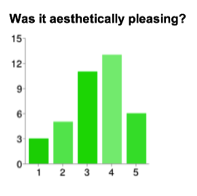
\includegraphics[scale=1]{Prototype/results.png}
\end{figure}

\subsection{Significant Changes in Capabilities}
Changes in prototype capabilities are listed below:\begin{itemize}
	\item Got rid of the tabbed layout in favor of a more focused main “home page” with less important screens being accessible from a side panel
	\item Support for linking additional tap accounts for the purpose of allowing dependents to be charged with one QR scan\\
	Eg: a mom would create tap accounts for her kids, links those accounts to her account through the app and then can use her phone to scan the kids in 
	\item App will use your location (updated ~every 2 minutes) to find the nearest metro line to location and will automatically display your ticket on the home screen 
	\item If GPS is off or you're using the bus, ability to manually choose a ticket from list as well 
	\item The home screen will display arrival times of the nearest train line to currently location along with destination of train
	\item Visually display any special statuses such as senior citizen, child or any discount passes
\end{itemize}

\clearpage

\subsection{Prototype Updates}
\begin{figure}[!htbp]
\centering
	\begin{subfigure}[t]{0.45\textwidth}
		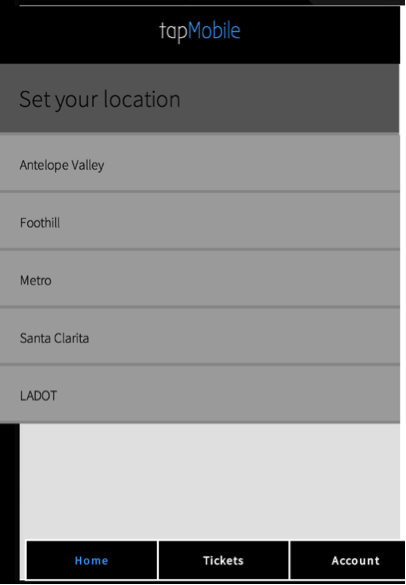
\includegraphics[scale=0.7]{Prototype/v1.png}
		\subcaption{Version 1}
	\end{subfigure}\begin{subfigure}[t]{0.45\textwidth}
		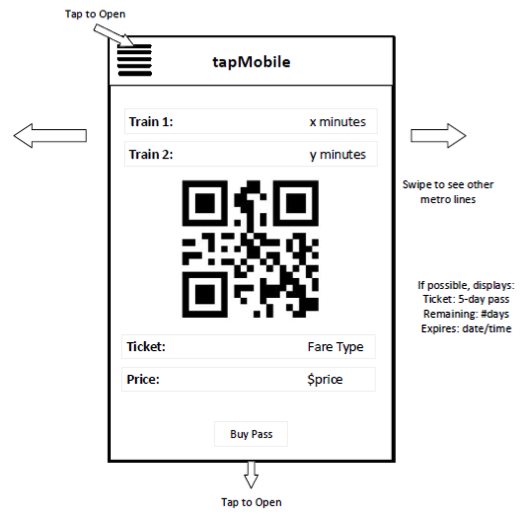
\includegraphics[scale=0.7]{Prototype/v2.png}
		\subcaption{Version 2}
	\end{subfigure}
\end{figure}

\begin{figure}
\centering
	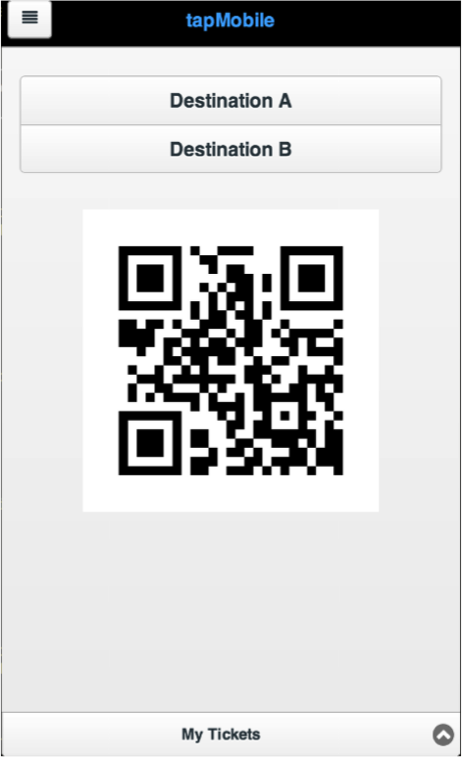
\includegraphics[scale=1]{Prototype/home.png}
\caption{Home Page}
\end{figure}

\begin{figure}
\centering
	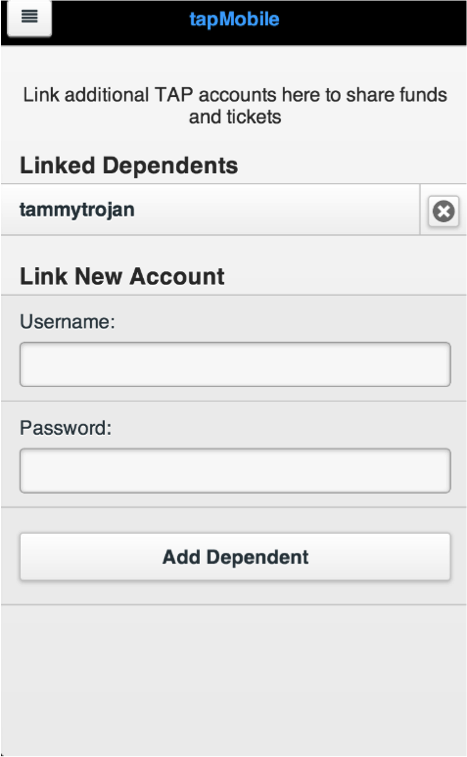
\includegraphics[scale=1]{Prototype/dependents.png}
\caption{Dependents Page}
\end{figure}

\begin{figure}
\centering
	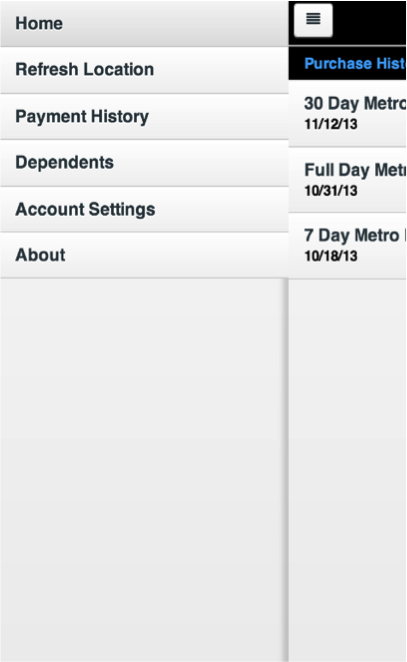
\includegraphics[scale=1]{Prototype/side-panel.png}
\caption{Side Panel}
\end{figure}